\documentclass[11pt,a4paper]{article}
\usepackage[utf8]{inputenc}
\usepackage[T1]{fontenc}
\usepackage[margin=2cm]{geometry}
\usepackage{booktabs}
\usepackage{array}
\usepackage{tikz}
\usetikzlibrary{arrows.meta,positioning,calc,shapes.geometric,circuits.logic.US}
\usepackage{xcolor}
\usepackage{pdflscape}
\usepackage{float}
\usepackage{amsmath}
\usepackage[colorlinks=true,urlcolor=blue!50!black,linkcolor=black]{hyperref}

\newcommand{\sig}[1]{\texttt{#1}}
\renewcommand{\arraystretch}{1.15}
\renewcommand{\figurename}{Figura}
\renewcommand{\tablename}{Tabla}
\renewcommand{\refname}{Referencias}

\tikzset{
  reg/.style={draw=teal!60!black,fill=teal!15,line width=0.5pt,align=center,font=\footnotesize},
  cmp/.style={draw=violet!60!black,fill=violet!12,line width=0.5pt,align=center,font=\footnotesize},
  muxs/.style={draw=gray!70!black,fill=gray!15,line width=0.5pt},
  ar/.style={-{Stealth[length=1.8mm]},line width=0.5pt},
  bus/.style={-{Stealth[length=2mm]},line width=1pt},
  ctl/.style={-{Stealth[length=1.6mm]},line width=0.4pt,draw=blue!60!black,dashed},
  pnl/.style={draw=gray!60,rounded corners=4pt,dashed,line width=0.5pt},
  lab/.style={font=\tiny},
  clab/.style={font=\tiny,text=blue!55!black}
}
% mux: nombre, x, y, alto, n entradas. Entradas: nombre-0.. (arriba a abajo), salida nombre-o, selector nombre-s
\newcommand{\mux}[5]{%
 \pgfmathtruncatemacro{\nmx}{#5-1}%
 \draw[muxs] (#2,#3+#4/2) -- (#2+0.7,#3+#4/2-0.4) -- (#2+0.7,#3-#4/2+0.4) -- (#2,#3-#4/2) -- cycle;
 \foreach \i in {0,...,\nmx}{%
   \pgfmathsetmacro{\oy}{((#5-1)/2-\i)*(#4/#5)}%
   \coordinate (#1-\i) at (#2,#3+\oy);}
 \coordinate (#1-o) at (#2+0.7,#3);
 \coordinate (#1-s) at (#2+0.35,#3-#4/2+0.2);}
\tikzset{
  and3/.style={and gate US,draw,line width=0.5pt,logic gate input sep=0.45cm,minimum height=1.2cm,minimum width=0.9cm},
  and2/.style={and gate US,draw,line width=0.5pt,logic gate input sep=0.45cm,minimum height=0.8cm,minimum width=0.85cm},
  or2/.style={or gate US,draw,line width=0.5pt,logic gate input sep=0.45cm,minimum height=0.8cm,minimum width=0.85cm}
}
\newcommand{\inp}[2]{\draw[ar] ([xshift=-0.6cm]#1) -- (#1) node[pos=0,left,lab]{#2};}
\newcommand{\outp}[2]{\draw[ar] (#1) -- ([xshift=0.6cm]#1) node[pos=1,right,lab]{#2};}
\newcommand{\ctl}[2]{\draw[ctl] ([yshift=-0.6cm]#1-s) -- (#1-s) node[pos=0,below,clab]{#2};}
\newcommand{\panel}[5]{\draw[pnl] (#1,#2) rectangle (#3,#4);
 \node[anchor=north west,font=\scriptsize\bfseries,text=gray!55!black] at (#1+0.1,#4-0.08) {#5};}
\newcommand{\clk}[1]{\draw[teal!60!black,line width=0.4pt] ([xshift=0.15cm]#1.south west) -- ++(0.1,0.17) -- ++(0.1,-0.17);}
\title{CPU S-MIPS multiciclo en Logisim\\[2pt]\large Datapath, codificaci\'on de estados y operaciones hacia la ALU}
\author{Roger Pe\~na P\'erez}
\date{22 de noviembre de 2026}
\begin{document}
\maketitle

\section{Operaciones que llegan a la ALU}
El \texttt{ALUOpEnc} es un priority encoder de 8 entradas; \sig{Eq} y \sig{bne} comparten la entrada 7.

\begin{table}[H]
\centering
\begin{tabular}{llp{6.3cm}}
\toprule
AluOp & Operaci\'on de la ALU & Instrucciones\\
\midrule
000 & $A+B$ & add, addu, addi, addiu, lw, lb, lbu, sw, sb\\
001 & $A-B$ & sub\\
010 & $A\land B$ & and, andi\\
011 & $A\lor B$ & or, ori\\
100 & $[A<B]$ (con signo) & slt, slti\\
101 & $B\ll A[4{:}0]$ & sll, lui\\
110 & $B\gg A[4{:}0]$ (l\'ogico) & srl\\
111 & $[A=B]$ & beq, bne\\
\bottomrule
\end{tabular}
\caption{Operaciones del decodificador hacia la ALU.}
\end{table}

\begin{itemize}
  \item $\sig{Zero}=[\text{Result}=0]$. Con AluOp = 111, \sig{Zero}=1 significa $A\neq B$.
  \item Opcodes: addi 08, addiu 09, slti 0A, andi 0C, ori 0D, lui 0F, lb 20, lw 23, lbu 24, sb 28, sw 2B, beq 04, bne 05, j 02, jal 03.
  \item Funct: sll 00, srl 02, jr 08, syscall 0C, add 20, addu 21, sub 22, and 24, or 25, slt 2A.
\end{itemize}


\section{Datapath}
\subsection{Vista general}
Tu Datapath est\'a organizado en ocho secciones, con los mismos nombres que usas en el circuito. La Figura~\ref{fig:general} muestra el orden en que viaja la informaci\'on: se lee la instrucci\'on, se extraen sus campos, se leen los registros, se eligen los operandos de la ALU, se calcula y el resultado vuelve al banco de registros, a la memoria o al PC.

\begin{landscape}
\begin{figure}[p]
\centering
\resizebox{\linewidth}{!}{%
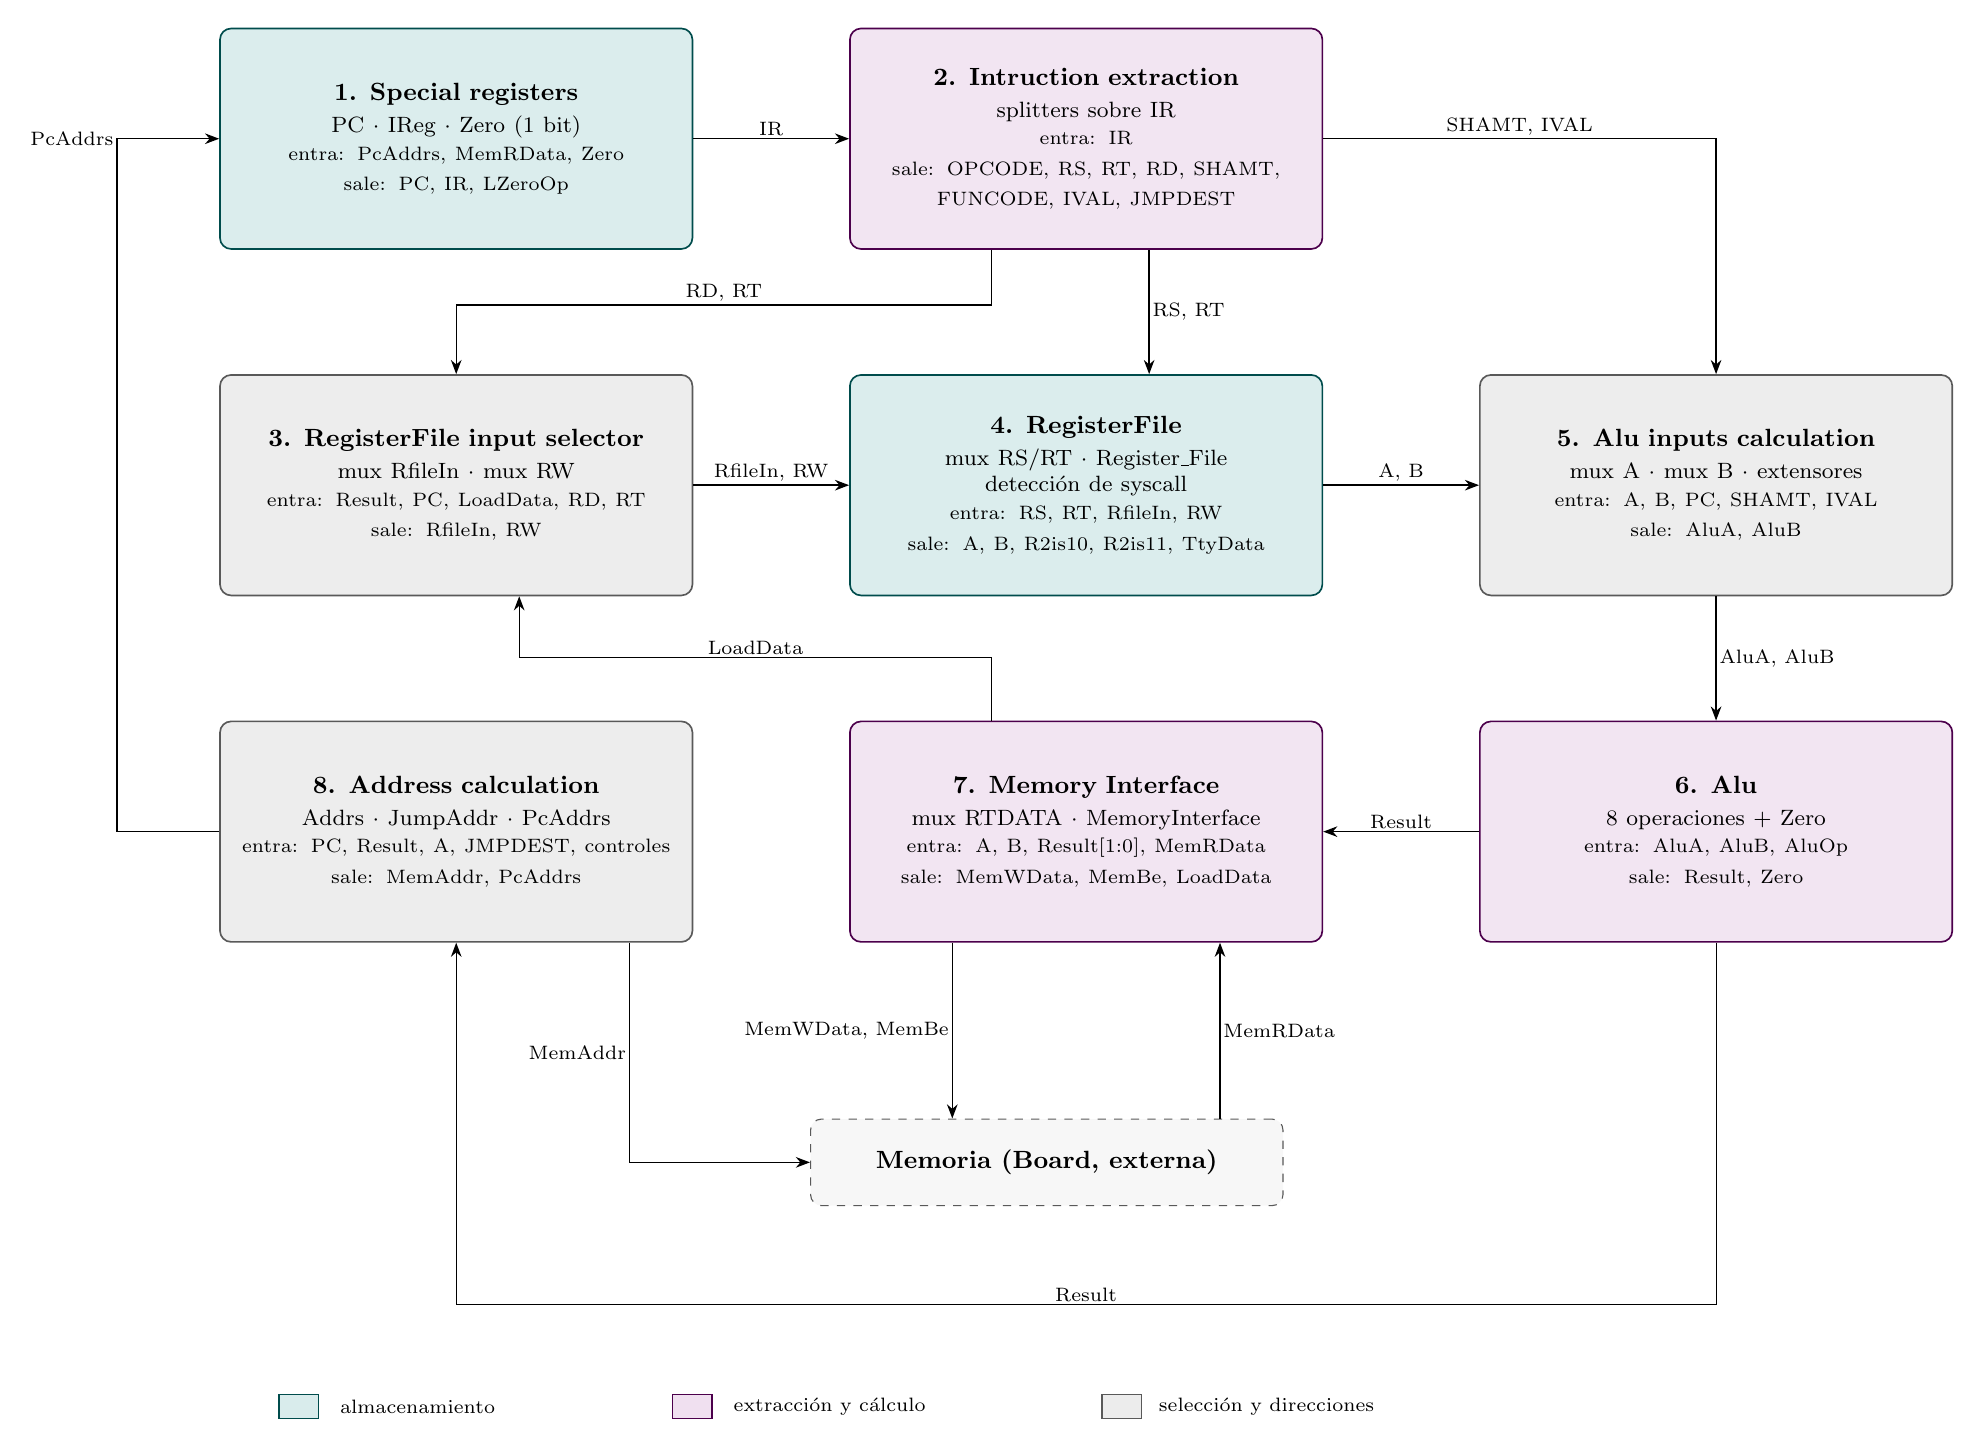
\begin{tikzpicture}[
  pb/.style={draw,rounded corners=4pt,minimum width=6cm,text width=5.5cm,minimum height=2.8cm,align=center,line width=0.6pt,font=\small,inner sep=4pt},
  pt/.style={pb,draw=teal!60!black,fill=teal!14},
  pv/.style={pb,draw=violet!60!black,fill=violet!10},
  pg/.style={pb,draw=gray!70!black,fill=gray!14},
  fl/.style={font=\scriptsize,fill=white,inner sep=1pt}
]
\node[pt] (p1) at (3,12)   {\textbf{1. Special registers}\\[2pt]\footnotesize PC $\cdot$ IReg $\cdot$ Zero (1 bit)\\[2pt]\scriptsize entra: PcAddrs, MemRData, Zero\\ sale: PC, IR, LZeroOp};
\node[pv] (p2) at (11,12)  {\textbf{2. Intruction extraction}\\[2pt]\footnotesize splitters sobre IR\\[2pt]\scriptsize entra: IR\\ sale: OPCODE, RS, RT, RD, SHAMT, FUNCODE, IVAL, JMPDEST};
\node[pg] (p3) at (3,7.6)  {\textbf{3. RegisterFile input selector}\\[2pt]\footnotesize mux RfileIn $\cdot$ mux RW\\[2pt]\scriptsize entra: Result, PC, LoadData, RD, RT\\ sale: RfileIn, RW};
\node[pt] (p4) at (11,7.6) {\textbf{4. RegisterFile}\\[2pt]\footnotesize mux RS/RT $\cdot$ Register\_File\\ detección de syscall\\[2pt]\scriptsize entra: RS, RT, RfileIn, RW\\ sale: A, B, R2is10, R2is11, TtyData};
\node[pg] (p5) at (19,7.6) {\textbf{5. Alu inputs calculation}\\[2pt]\footnotesize mux A $\cdot$ mux B $\cdot$ extensores\\[2pt]\scriptsize entra: A, B, PC, SHAMT, IVAL\\ sale: AluA, AluB};
\node[pv] (p6) at (19,3.2) {\textbf{6. Alu}\\[2pt]\footnotesize 8 operaciones + Zero\\[2pt]\scriptsize entra: AluA, AluB, AluOp\\ sale: Result, Zero};
\node[pv] (p7) at (11,3.2) {\textbf{7. Memory Interface}\\[2pt]\footnotesize mux RTDATA $\cdot$ MemoryInterface\\[2pt]\scriptsize entra: A, B, Result[1:0], MemRData\\ sale: MemWData, MemBe, LoadData};
\node[pg] (p8) at (3,3.2)  {\textbf{8. Address calculation}\\[2pt]\footnotesize Addrs $\cdot$ JumpAddr $\cdot$ PcAddrs\\[2pt]\scriptsize entra: PC, Result, A, JMPDEST, controles\\ sale: MemAddr, PcAddrs};
\node[draw=gray!70!black,dashed,fill=gray!6,rounded corners=4pt,minimum width=6cm,minimum height=1.1cm,font=\small] (mem) at (10.5,-1.0) {\textbf{Memoria (Board, externa)}};
% flechas principales
\draw[ar] (p1.east) -- (p2.west) node[midway,above,fl]{IR};
\draw[ar] ([xshift=0.8cm]p2.south) -- ([xshift=0.8cm]p4.north) node[midway,right,fl]{RS, RT};
\draw[ar] ([xshift=-1.2cm]p2.south) -- ++(0,-0.7) -| (p3.north) node[pos=0.25,above,fl]{RD, RT};
\draw[ar] (p2.east) -| (p5.north) node[pos=0.25,above,fl]{SHAMT, IVAL};
\draw[ar] (p3.east) -- (p4.west) node[midway,above,fl]{RfileIn, RW};
\draw[ar] (p4.east) -- (p5.west) node[midway,above,fl]{A, B};
\draw[ar] (p5.south) -- (p6.north) node[midway,right,fl]{AluA, AluB};
\draw[ar] (p6.west) -- (p7.east) node[midway,above,fl]{Result};
\draw[ar] ([xshift=-1.2cm]p7.north) -- ++(0,0.8) -| ([xshift=0.8cm]p3.south) node[pos=0.25,above,fl]{LoadData};
\draw (p6.south) -- ++(0,-4.6) coordinate (r1);
\draw (r1) -- (r1 -| p8.south) coordinate (r2);
\draw[ar] (r2) -- (p8.south);
\node[fl,above] at ($(r1)!0.5!(r2)$) {Result};
\draw[ar] (p8.west) -- ++(-1.3,0) |- (p1.west) node[midway,left,fl]{PcAddrs};
\draw[ar] ($(p7.south)+(-1.7,0)$) -- ($(mem.north -| p7.south)+(-1.7,0)$) node[midway,left,fl]{MemWData, MemBe};
\draw[ar] ($(mem.north -| p7.south)+(1.7,0)$) -- ($(p7.south)+(1.7,0)$) node[midway,right,fl]{MemRData};
\draw[ar] ($(p8.south)+(2.2,0)$) |- (mem.west) node[pos=0.25,left,fl]{MemAddr};
% leyenda
\node[reg,minimum width=0.5cm,minimum height=0.3cm] at (1,-4.1) {};
\node[anchor=west,font=\scriptsize] at (1.4,-4.1) {almacenamiento};
\node[cmp,minimum width=0.5cm,minimum height=0.3cm] at (6,-4.1) {};
\node[anchor=west,font=\scriptsize] at (6.4,-4.1) {extracci\'on y c\'alculo};
\draw[muxs] (11.2,-4.25) rectangle (11.7,-3.95);
\node[anchor=west,font=\scriptsize] at (11.8,-4.1) {selecci\'on y direcciones};
\end{tikzpicture}}
\caption{Vista general del Datapath, con las ocho secciones de tu circuito. Las flechas son el flujo principal; PC, Result, A, B y las se\~nales de control viajan por tunnels (ver Tabla~\ref{tab:puertos} y las figuras siguientes).}
\label{fig:general}
\end{figure}
\end{landscape}


\subsection{Secci\'on por secci\'on}
\paragraph{1. Special registers y 2. Intruction extraction.}
\begin{itemize}
  \item \textbf{PC}: 32 bits, $D=\sig{PcAddrs}$, $EN=\sig{PCEN}$.
  \item \textbf{IReg}: 32 bits, $D=\sig{MemRData}$, $EN=\sig{IRwrite}$ (que es \sig{InFetch}); la instrucci\'on queda guardada al final de Fetch.
  \item \textbf{Zero}: registro de 1 bit sin \texttt{EN}: guarda el \sig{Zero} de la ALU en cada ciclo. En Branch, \sig{LZeroOp} conserva lo que la ALU calcul\'o en Decode (con AluOp = 111, $\sig{Zero}=0$ significa $A=B$).
  \item Los splitters del IR producen los campos de la Tabla~\ref{tab:campos}.
\end{itemize}
\begin{figure}[H]
\centering
\resizebox{\linewidth}{!}{%
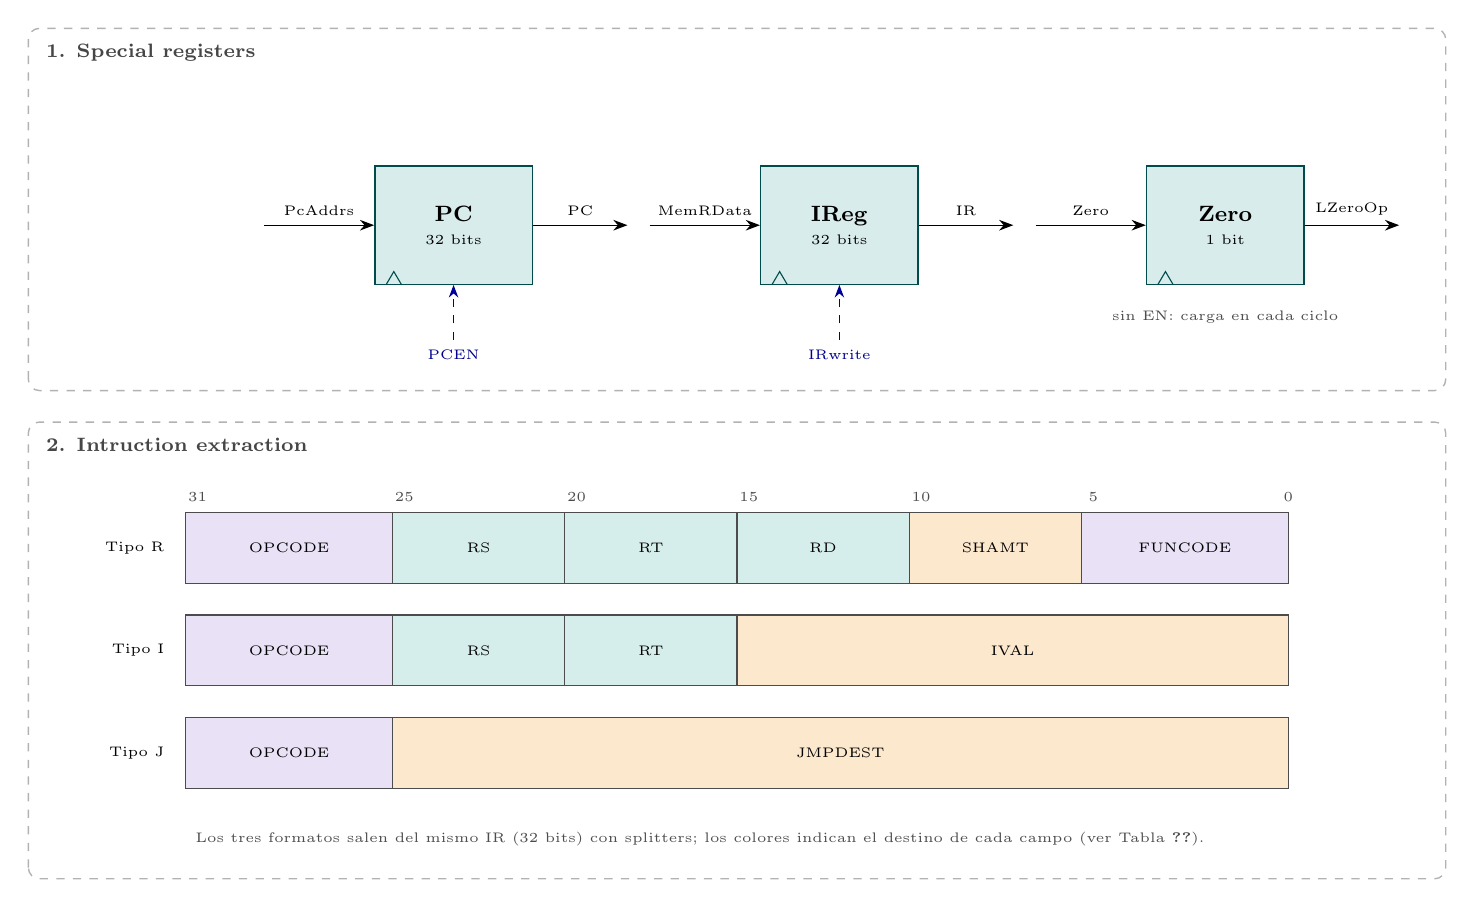
\begin{tikzpicture}
\panel{-2}{6.2}{16}{10.8}{1. Special registers}
\node[reg,minimum width=2cm,minimum height=1.5cm] (pc) at (3.4,8.3) {\textbf{PC}\\[-1pt]\tiny 32 bits};
\node[reg,minimum width=2cm,minimum height=1.5cm] (ir) at (8.3,8.3) {\textbf{IReg}\\[-1pt]\tiny 32 bits};
\node[reg,minimum width=2cm,minimum height=1.5cm] (zr) at (13.2,8.3) {\textbf{Zero}\\[-1pt]\tiny 1 bit};
\clk{pc}\clk{ir}\clk{zr}
\draw[ar] ([xshift=-1.4cm]pc.west) -- (pc.west) node[midway,above,lab]{PcAddrs};
\draw[ar] (pc.east) -- ++(1.2,0) node[midway,above,lab]{PC};
\draw[ar] ([xshift=-1.4cm]ir.west) -- (ir.west) node[midway,above,lab]{MemRData};
\draw[ar] (ir.east) -- ++(1.2,0) node[midway,above,lab]{IR};
\draw[ar] ([xshift=-1.4cm]zr.west) -- (zr.west) node[midway,above,lab]{Zero};
\draw[ar] (zr.east) -- ++(1.2,0) node[midway,above,lab]{LZeroOp};
\draw[ctl] ([yshift=-0.7cm]pc.south) -- (pc.south) node[pos=0,below,clab]{PCEN};
\draw[ctl] ([yshift=-0.7cm]ir.south) -- (ir.south) node[pos=0,below,clab]{IRwrite};
\node[font=\tiny,text=gray!60!black,below] at ([yshift=-0.2cm]zr.south) {sin EN: carga en cada ciclo};
%
\panel{-2}{0}{16}{5.8}{2. Intruction extraction}
\def\bw{0.4375}
\newcommand{\fld}[5]{\draw[fill=#5,draw=gray!60!black,line width=0.4pt] (#1*\bw,#3-0.45) rectangle (#2*\bw,#3+0.45);
  \node[font=\tiny] at ({(#1+#2)*\bw/2},#3) {#4};}
\definecolor{fdec}{RGB}{233,225,246}
\definecolor{freg}{RGB}{214,238,235}
\definecolor{fimm}{RGB}{252,232,205}
\node[font=\tiny,anchor=east] at (-0.15,4.2) {Tipo R};
\fld{0}{6}{4.2}{OPCODE}{fdec}\fld{6}{11}{4.2}{RS}{freg}\fld{11}{16}{4.2}{RT}{freg}\fld{16}{21}{4.2}{RD}{freg}\fld{21}{26}{4.2}{SHAMT}{fimm}\fld{26}{32}{4.2}{FUNCODE}{fdec}
\node[font=\tiny,anchor=east] at (-0.15,2.9) {Tipo I};
\fld{0}{6}{2.9}{OPCODE}{fdec}\fld{6}{11}{2.9}{RS}{freg}\fld{11}{16}{2.9}{RT}{freg}\fld{16}{32}{2.9}{IVAL}{fimm}
\node[font=\tiny,anchor=east] at (-0.15,1.6) {Tipo J};
\fld{0}{6}{1.6}{OPCODE}{fdec}\fld{6}{32}{1.6}{JMPDEST}{fimm}
\foreach \b/\x in {31/0,25/6,20/11,15/16,10/21,5/26}{\node[font=\tiny,text=gray!60!black] at ({\x*\bw+0.15},4.85) {\b};}
\node[font=\tiny,text=gray!60!black] at (14.0,4.85) {0};
\node[font=\tiny,text=gray!60!black,anchor=west] at (0,0.5) {Los tres formatos salen del mismo IR (32 bits) con splitters; los colores indican el destino de cada campo (ver Tabla~\ref{tab:campos}).};
\end{tikzpicture}}
\caption{Secciones 1 y 2: registros especiales y extracci\'on de campos de la instrucci\'on.}
\label{fig:s12}
\end{figure}

\begin{table}[H]
\centering
\small
\begin{tabular}{lll}
\toprule
Campo & Bits & Destino\\
\midrule
OPCODE & 31--26 & pin \sig{Opcode} $\to$ Instruction\_Decoder\\
FUNCODE & 5--0 & pin \sig{Funct} $\to$ Instruction\_Decoder\\
RS, RT, RD & 25--21, 20--16, 15--11 & secciones 3 y 4 (direcciones de registros)\\
SHAMT & 10--6 & Extender5B (secci\'on 5)\\
IVAL & 15--0 & Extender16B (secci\'on 5)\\
JMPDEST & 25--0 & JumpAddr (secci\'on 8)\\
\bottomrule
\end{tabular}
\caption{Campos extra\'idos del IR y su destino.}
\label{tab:campos}
\end{table}

\paragraph{3. RegisterFile input selector y 4. RegisterFile.}
\begin{itemize}
  \item $\sig{RfileIn}=\sig{Mem2Reg}\ ?\ \sig{LoadData} : (\sig{Jal}\ ?\ \mathrm{PC} : \mathrm{Result})$. Con \sig{Jal} se guarda el PC (ya incrementado en Fetch) en \$31.
  \item \sig{RW} elige el registro destino: RD, RT o \$31 seg\'un $\sig{SaveReg}=0,1,3$ (la entrada 2 no est\'a conectada).
  \item Con \sig{SysCall}, los muxes de lectura reemplazan RS por 2 (\$v0) y RT por 4 (\$a0): as\'i $A=\$v0$ y $B=\$a0$.
  \item $\sig{R2is10}=\sig{SysCall}\land(A=10)$ (salir) y $\sig{R2is11}=\sig{SysCall}\land(A=11)$ (imprimir); $\sig{TtyData}=B[6{:}0]$.
\end{itemize}
\begin{figure}[H]
\centering
\resizebox{\linewidth}{!}{%
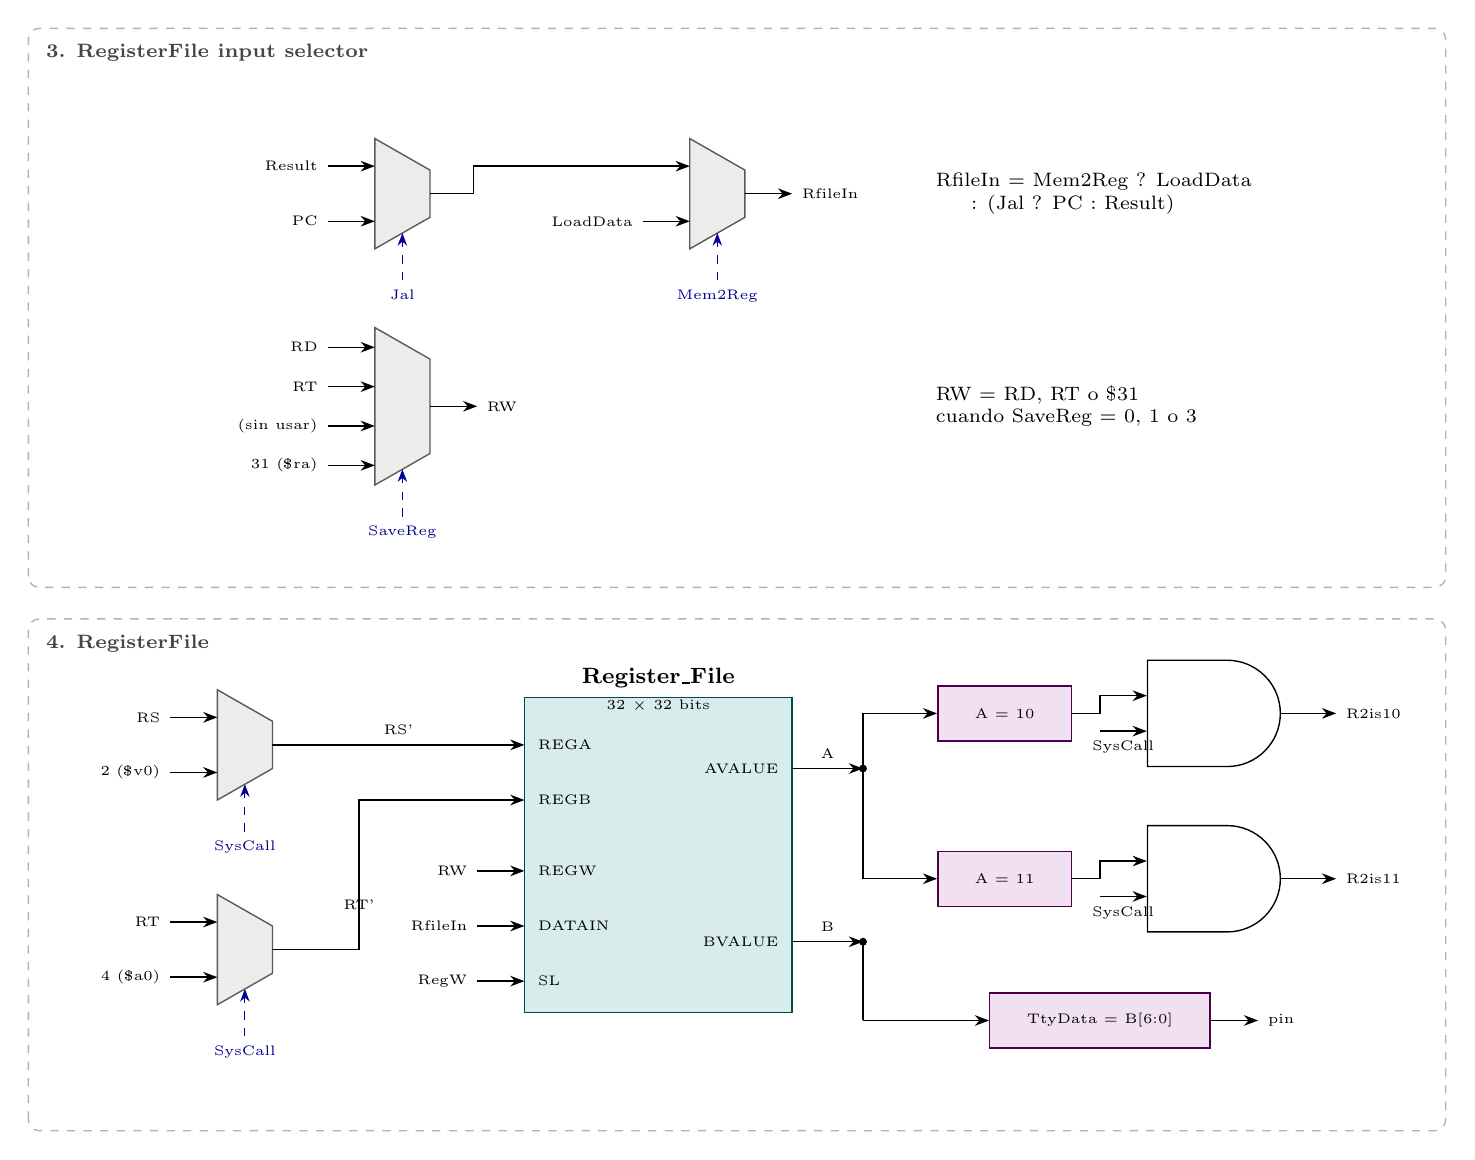
\begin{tikzpicture}
\panel{-2}{6.3}{16}{13.4}{3. RegisterFile input selector}
\mux{mj}{2.4}{11.3}{1.4}{2}
\inp{mj-0}{Result}\inp{mj-1}{PC}\ctl{mj}{Jal}
\mux{mm}{6.4}{11.3}{1.4}{2}
\draw[ar] (mj-o) -- ++(0.55,0) |- (mm-0);
\inp{mm-1}{LoadData}\ctl{mm}{Mem2Reg}\outp{mm-o}{RfileIn}
\mux{mw}{2.4}{8.6}{2.0}{4}
\inp{mw-0}{RD}\inp{mw-1}{RT}\inp{mw-2}{(sin usar)}\inp{mw-3}{31 (\$ra)}\ctl{mw}{SaveReg}\outp{mw-o}{RW}
\node[anchor=west,font=\scriptsize,align=left] at (9.4,11.3) {RfileIn = Mem2Reg ? LoadData\\ \hspace*{1.6em}: (Jal ? PC : Result)};
\node[anchor=west,font=\scriptsize,align=left] at (9.4,8.6) {RW = RD, RT o \$31\\ cuando SaveReg = 0, 1 o 3};
%
\panel{-2}{-0.6}{16}{5.9}{4. RegisterFile}
\mux{ms}{0.4}{4.3}{1.4}{2}
\inp{ms-0}{RS}\inp{ms-1}{2 (\$v0)}\ctl{ms}{SysCall}
\mux{mt}{0.4}{1.7}{1.4}{2}
\inp{mt-0}{RT}\inp{mt-1}{4 (\$a0)}\ctl{mt}{SysCall}
\node[reg,minimum width=3.4cm,minimum height=4.0cm] (rf) at (6.0,2.9) {};
\node[font=\footnotesize\bfseries] at (6.0,5.15) {Register\_File};
\node[font=\tiny] at (6.0,4.8) {32 $\times$ 32 bits};
\foreach \y/\n in {4.3/REGA,3.6/REGB,2.7/REGW,2.0/DATAIN,1.3/SL}{\node[font=\tiny,anchor=west] at (4.35,\y) {\n};}
\foreach \y/\n in {4.0/AVALUE,1.8/BVALUE}{\node[font=\tiny,anchor=east] at (7.65,\y) {\n};}
\draw[ar] (ms-o) -- (4.3,4.3) node[pos=0.5,above,lab]{RS'};
\draw[ar] (mt-o) -- (2.2,1.7) |- (4.3,3.6) node[pos=0.1,above,lab]{RT'};
\draw[ar] (3.7,2.7) -- (4.3,2.7) node[pos=0,left,lab]{RW};
\draw[ar] (3.7,2.0) -- (4.3,2.0) node[pos=0,left,lab]{RfileIn};
\draw[ar] (3.7,1.3) -- (4.3,1.3) node[pos=0,left,lab]{RegW};
\draw[ar] (7.7,4.0) -- ++(0.9,0) node[pos=0.5,above,lab]{A};
\draw[ar] (7.7,1.8) -- ++(0.9,0) node[pos=0.5,above,lab]{B};
% deteccion de syscall
\fill (8.6,4.0) circle (0.05);
\node[cmp,minimum width=1.7cm,minimum height=0.7cm] (c10) at (10.4,4.7) {\tiny A = 10};
\node[cmp,minimum width=1.7cm,minimum height=0.7cm] (c11) at (10.4,2.6) {\tiny A = 11};
\draw[ar] (8.6,4.0) |- (c10.west);
\draw[ar] (8.6,4.0) |- (c11.west);
\node[and2,logic gate inputs=nn] (g10) at (13.0,4.7) {};
\node[and2,logic gate inputs=nn] (g11) at (13.0,2.6) {};
\draw[ar] (c10.east) -- ++(0.35,0) |- (g10.input 1);
\draw[ar] (c11.east) -- ++(0.35,0) |- (g11.input 1);
\draw[ar] ([xshift=-0.6cm]g10.input 2) -- (g10.input 2) node[pos=0.5,below,lab]{SysCall};
\draw[ar] ([xshift=-0.6cm]g11.input 2) -- (g11.input 2) node[pos=0.5,below,lab]{SysCall};
\draw[ar] (g10.output) -- ++(0.7,0) node[right,lab]{R2is10};
\draw[ar] (g11.output) -- ++(0.7,0) node[right,lab]{R2is11};
\draw (8.6,1.8) -- (8.6,0.8);
\draw[ar] (8.6,0.8) -- (10.2,0.8);
\fill (8.6,1.8) circle (0.05);
\node[cmp,minimum width=2.8cm,minimum height=0.7cm,anchor=west] (tty) at (10.2,0.8) {\tiny TtyData = B[6:0]};
\draw[ar] (tty.east) -- ++(0.6,0) node[right,lab]{pin};
\end{tikzpicture}}
\caption{Secciones 3 y 4: selector de entrada del banco de registros y banco de registros (con la lectura de \$v0/\$a0 para syscall).}
\label{fig:s34}
\end{figure}


\paragraph{5. Alu inputs calculation y 6. Alu.}
\begin{itemize}
  \item \sig{ABSrc} se divide en $\sig{ASel}=\sig{ABSrc}[1{:}0]$ y $\sig{BSel}=\sig{ABSrc}[3{:}2]$.
  \item \textbf{Mux A} (ASel): 0 = A, 1 = PC, 2 = shamt extendido con ceros, 3 = 16
  \item \textbf{Mux B} (BSel): 0 = B, 1 = 4, 2 = \sig{IValExt}, 3 = $\sig{IValExt}\ll2$ (desplazamiento de saltos).
  \item \sig{IValExt} extiende IVAL con signo si $\sig{Sign}=1$ y con ceros si no.
  \item La ALU recibe \sig{AluA}, \sig{AluB} y \sig{AluOp}; devuelve \sig{Result} y $\sig{Zero}=[\mathrm{Result}=0]$.
\end{itemize}
\begin{figure}[H]
\centering
\resizebox{\linewidth}{!}{%
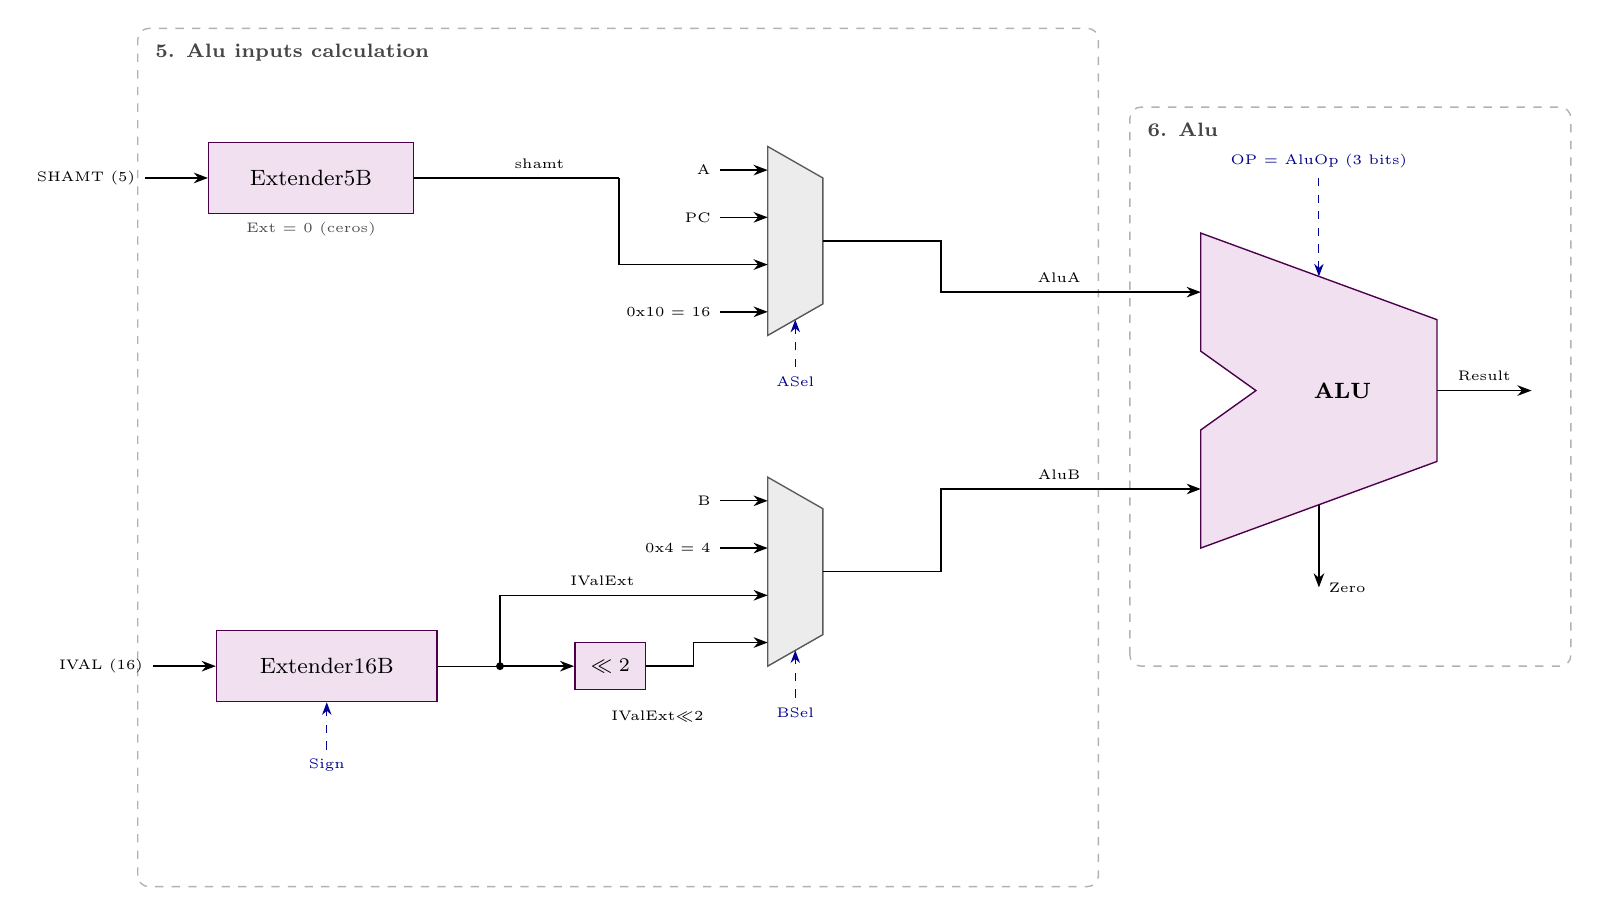
\begin{tikzpicture}
\panel{-2}{-0.6}{10.2}{10.3}{5. Alu inputs calculation}
\panel{10.6}{2.2}{16.2}{9.3}{6. Alu}
\node[cmp,minimum width=2.6cm,minimum height=0.9cm] (e5) at (0.2,8.4) {Extender5B};
\draw[ar] ([xshift=-0.8cm]e5.west) -- (e5.west) node[pos=0,left,lab]{SHAMT (5)};
\node[font=\tiny,text=gray!60!black] at (0.2,7.75) {Ext = 0 (ceros)};
\node[cmp,minimum width=2.8cm,minimum height=0.9cm] (e16) at (0.4,2.2) {Extender16B};
\draw[ar] ([xshift=-0.8cm]e16.west) -- (e16.west) node[pos=0,left,lab]{IVAL (16)};
\draw[ctl] ([yshift=-0.6cm]e16.south) -- (e16.south) node[pos=0,below,clab]{Sign};
\mux{xa}{6.0}{7.6}{2.4}{4}
\inp{xa-0}{A}\inp{xa-1}{PC}\inp{xa-3}{0x10 = 16}\ctl{xa}{ASel}
\draw (e5.east) -- ++(2.6,0) coordinate (q1);
\draw[ar] (q1) |- (xa-2);
\node[lab,above] at (3.1,8.4) {shamt};
\mux{xb}{6.0}{3.4}{2.4}{4}
\inp{xb-0}{B}\inp{xb-1}{0x4 = 4}\ctl{xb}{BSel}
\draw (e16.east) -- (2.6,2.2);
\fill (2.6,2.2) circle (0.05);
\draw[ar] (2.6,2.2) |- (xb-2);
\node[lab,above] at (3.9,3.1) {IValExt};
\node[cmp,minimum width=0.9cm,minimum height=0.6cm] (sh) at (4.0,2.2) {\scriptsize $\ll 2$};
\draw[ar] (2.6,2.2) -- (sh.west);
\draw[ar] (sh.east) -- ++(0.6,0) |- (xb-3);
\node[lab,below] at (4.6,1.75) {IValExt$\ll$2};
\draw[ar] (xa-o) -- ++(1.5,0) |- (11.5,6.95);
\draw[ar] (xb-o) -- ++(1.5,0) |- (11.5,4.45);
\node[lab,above] at (9.7,6.95) {AluA};
\node[lab,above] at (9.7,4.45) {AluB};
\draw[cmp] (11.5,7.7) -- (14.5,6.6) -- (14.5,4.8) -- (11.5,3.7) -- (11.5,5.2) -- (12.2,5.7) -- (11.5,6.2) -- cycle;
\node[font=\footnotesize\bfseries] at (13.3,5.7) {ALU};
\draw[ctl] (13.0,8.4) -- (13.0,7.15) node[pos=0,above,clab]{OP = AluOp (3 bits)};
\draw[ar] (14.5,5.7) -- (15.7,5.7) node[pos=0.5,above,lab]{Result};
\draw[ar] (13.0,4.25) -- (13.0,3.2) node[pos=1,right,lab]{Zero};
\end{tikzpicture}}
\caption{Secciones 5 y 6: selecci\'on de los operandos de la ALU (ASel y BSel) y la ALU.}
\label{fig:s56}
\end{figure}

\begin{figure}[H]
\centering
\resizebox{\linewidth}{!}{%
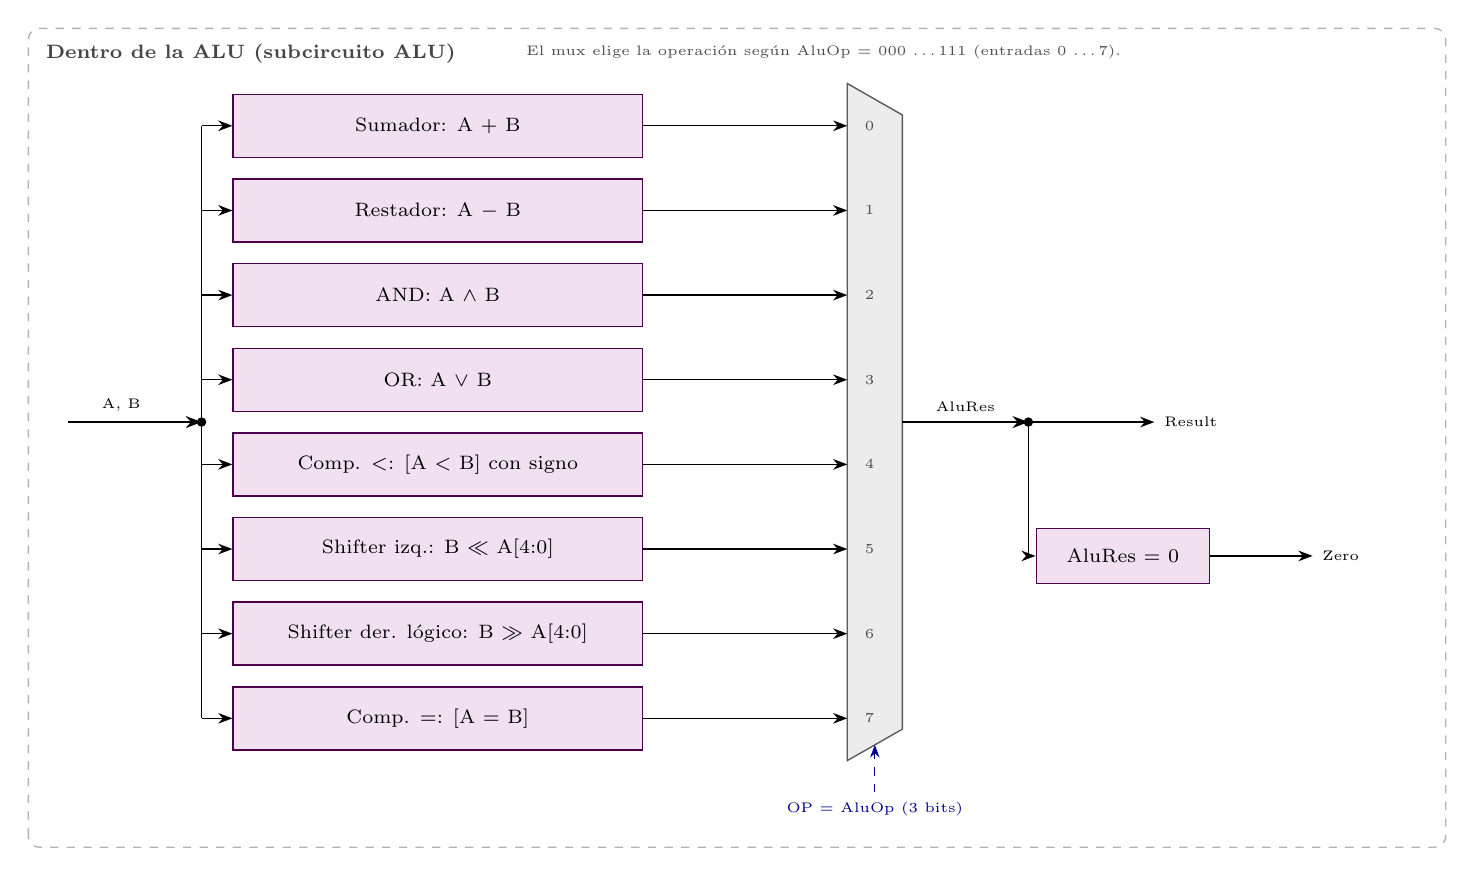
\begin{tikzpicture}
\panel{-2}{0}{16}{10.4}{Dentro de la ALU (subcircuito ALU)}
\mux{mo}{8.4}{5.4}{8.6}{8}
\foreach \i/\t in {0/{Sumador: A + B},1/{Restador: A $-$ B},2/{AND: A $\wedge$ B},3/{OR: A $\vee$ B},4/{Comp. $<$: [A $<$ B] con signo},5/{Shifter izq.: B $\ll$ A[4:0]},6/{Shifter der. l\'ogico: B $\gg$ A[4:0]},7/{Comp. $=$: [A = B]}}{
  \pgfmathsetmacro{\yy}{5.4+(3.5-\i)*1.075}
  \node[cmp,minimum width=5.2cm,minimum height=0.8cm,font=\scriptsize] (u\i) at (3.2,\yy) {\t};
  \draw[ar] (u\i.east) -- (mo-\i);
  \node[font=\tiny,text=gray!60!black,anchor=west] at (8.5,\yy) {\i};
  \draw[ar] (0.2,\yy) -- (u\i.west);
}
\draw (0.2,1.64) -- (0.2,9.16);
\draw[bus] (-1.5,5.4) -- (0.2,5.4) node[pos=0.4,above,lab]{A, B};
\fill (0.2,5.4) circle (0.06);
\ctl{mo}{OP = AluOp (3 bits)}
\draw[bus] (mo-o) -- ++(1.6,0) coordinate (rr) node[pos=0.5,above,lab]{AluRes};
\draw[ar] (rr) -- ++(1.6,0) node[right,lab]{Result};
\draw (rr) -- (rr |- 0,3.7);
\fill (rr) circle (0.06);
\node[cmp,minimum width=2.2cm,minimum height=0.7cm] (zz) at (11.9,3.7) {\scriptsize AluRes = 0};
\draw[ar] (rr |- 0,3.7) -- (zz.west);
\draw[ar] (zz.east) -- ++(1.3,0) node[right,lab]{Zero};
\node[font=\tiny,anchor=west,text=gray!60!black] at (4.2,10.1) {El mux elige la operaci\'on seg\'un AluOp = 000 \dots 111 (entradas 0 \dots 7).};
\end{tikzpicture}}
\caption{Estructura interna de la ALU: ocho unidades en paralelo, un mux de 8 entradas controlado por AluOp y el comparador contra cero que genera Zero.}
\label{fig:alu}
\end{figure}


\paragraph{7. Memory Interface y 8. Address calculation.}
\begin{itemize}
  \item $\mathrm{RTDATA}=\sig{Reg2Mem}\ ?\ B : A$ (en la pr\'actica, el dato a escribir es B); el offset es $\mathrm{Result}[1{:}0]$. \texttt{MemoryInterface} produce \sig{MemWData} y \sig{MemBe} para escrituras y \sig{LoadData} para lecturas (de palabra, o de byte con o sin signo seg\'un \sig{IsByte} y \sig{Sign}).
  \item $\sig{Addrs}=(\sig{Mem2Reg}\lor\sig{Reg2Mem})\ ?\ \mathrm{Result} : \mathrm{PC}$ y sale por el pin \sig{MemAddr}.
  \item $\sig{JumpAddr}=\mathrm{Result}[31{:}28]\,\|\,\sig{JMPDEST}\,\|\,00$. En el estado Jump, Result vale $\mathrm{PC}+4$, de ah\'i salen los 4 bits altos.
  \item $\sig{PcAddrs}=\sig{Jr}\ ?\ A : \bigl(\mathrm{mantener}\ ?\ \mathrm{PC} : (\sig{IsJump}\ ?\ \sig{JumpAddr} : \mathrm{Result})\bigr)$.
  \item $\mathrm{mantener}=\sig{PCsrc}\land\lnot\mathrm{bne\_tomado}\land\lnot\mathrm{beq\_tomado}$, con $\sig{PCsrc}=\sig{AddrSrc}$ de la ControlUnit ($0$ solo en Fetch y Jump) y $\sig{IsBranch}=\sig{InBranchState}$. Por eso, en cualquier otro estado el PC se recarga con su mismo valor salvo en un salto tomado; esto hace inofensivos los t\'erminos extra de \sig{PCEN} en \texttt{Branch\_Control} ($\sig{J}$, $\sig{Jr}$, $\sig{Beq}\land\lnot\sig{Zero}$, $\sig{Bne}\land\sig{Zero}$).
\end{itemize}
\begin{figure}[H]
\centering
\resizebox{\linewidth}{!}{%
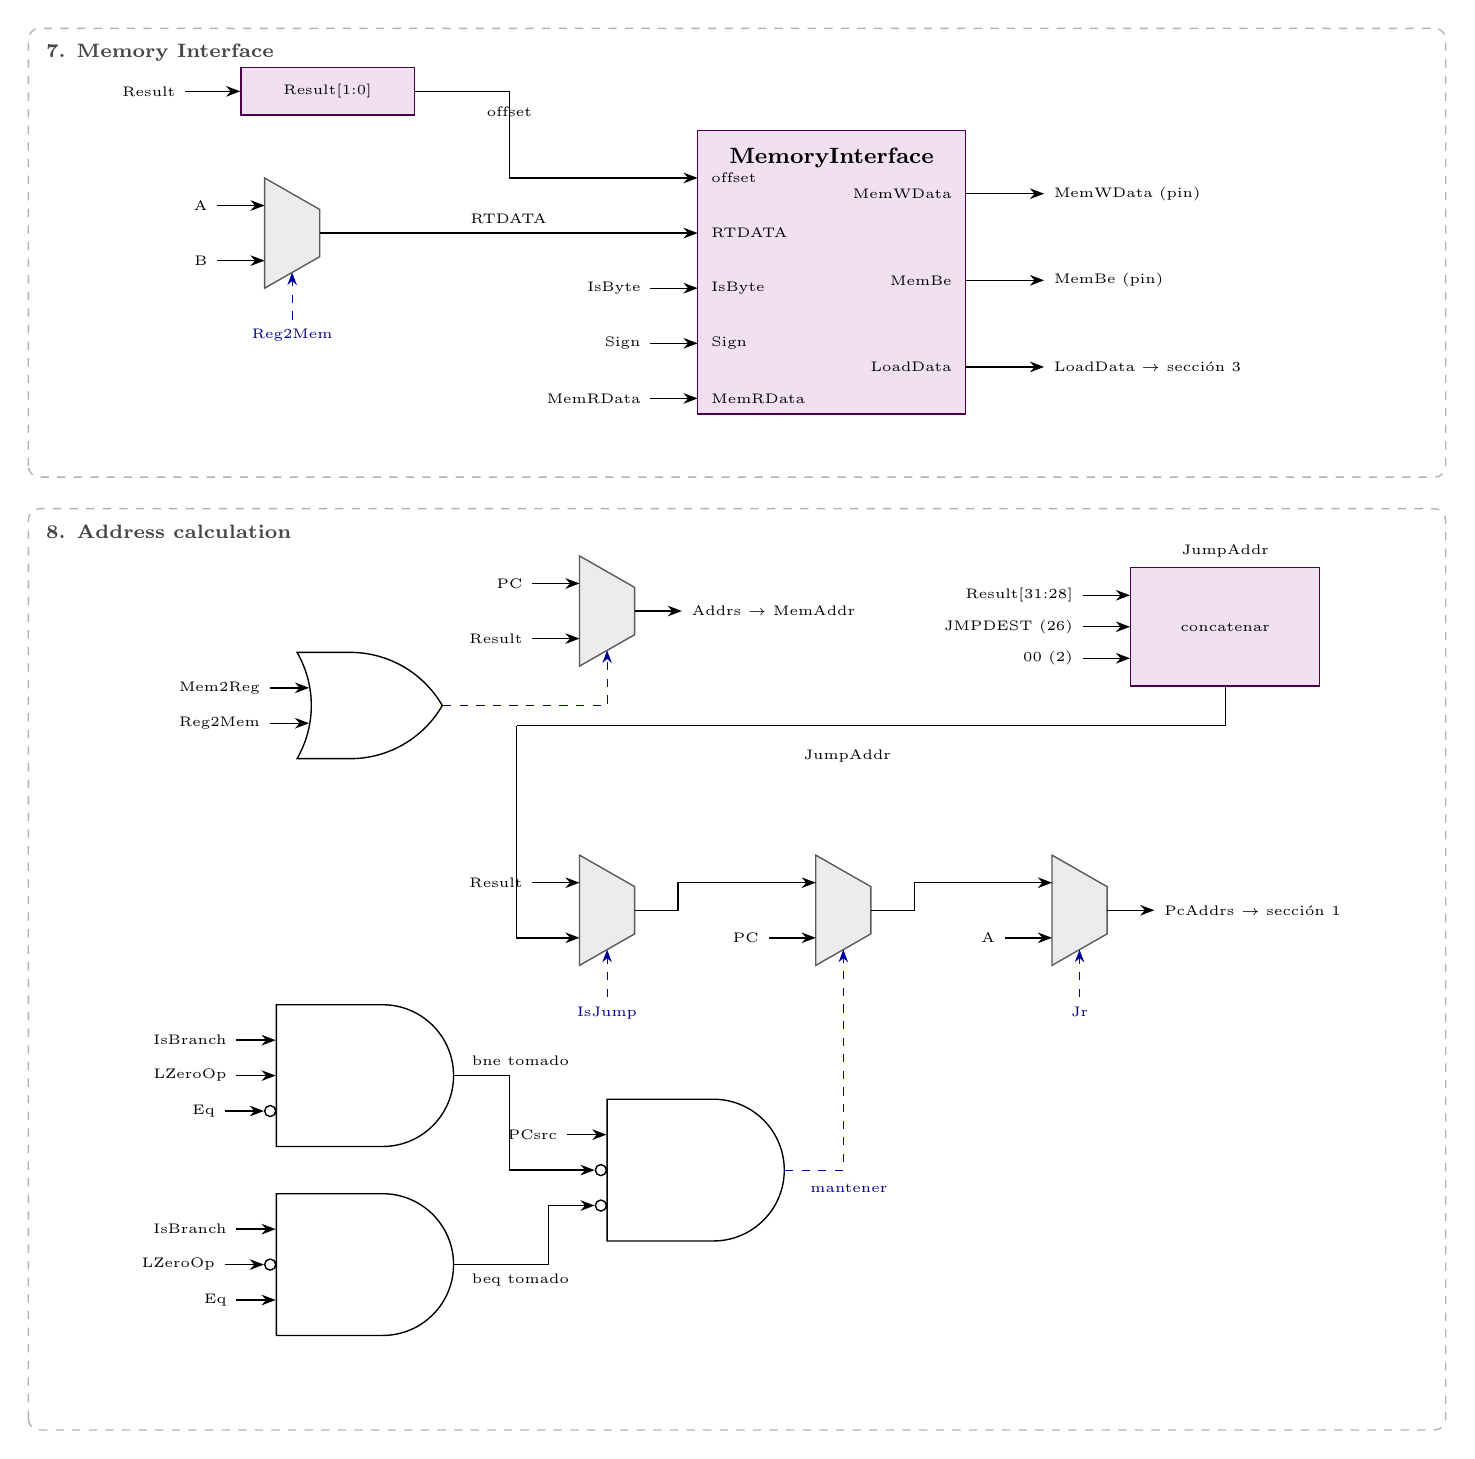
\begin{tikzpicture}
\panel{-2}{8.1}{16}{13.8}{7. Memory Interface}
\node[cmp,minimum width=2.2cm,minimum height=0.6cm] (off) at (1.8,13.0) {\tiny Result[1:0]};
\draw[ar] ([xshift=-0.7cm]off.west) -- (off.west) node[pos=0,left,lab]{Result};
\mux{md}{1.0}{11.2}{1.4}{2}
\inp{md-0}{A}\inp{md-1}{B}\ctl{md}{Reg2Mem}
\node[cmp,minimum width=3.4cm,minimum height=3.6cm] (mi) at (8.2,10.7) {};
\node[font=\footnotesize\bfseries] at (8.2,12.15) {MemoryInterface};
\foreach \y/\n in {11.9/offset,11.2/RTDATA,10.5/IsByte,9.8/Sign,9.1/MemRData}{\node[font=\tiny,anchor=west] at (6.55,\y) {\n};}
\foreach \y/\n in {11.7/MemWData,10.6/MemBe,9.5/LoadData}{\node[font=\tiny,anchor=east] at (9.85,\y) {\n};}
\draw[ar] (off.east) -- ++(1.2,0) |- (6.5,11.9) node[pos=0.2,above,lab]{offset};
\draw[ar] (md-o) -- (6.5,11.2) node[pos=0.5,above,lab]{RTDATA};
\draw[ar] (5.9,10.5) -- (6.5,10.5) node[pos=0,left,lab]{IsByte};
\draw[ar] (5.9,9.8) -- (6.5,9.8) node[pos=0,left,lab]{Sign};
\draw[ar] (5.9,9.1) -- (6.5,9.1) node[pos=0,left,lab]{MemRData};
\draw[ar] (9.9,11.7) -- ++(1.0,0) node[right,lab]{MemWData (pin)};
\draw[ar] (9.9,10.6) -- ++(1.0,0) node[right,lab]{MemBe (pin)};
\draw[ar] (9.9,9.5) -- ++(1.0,0) node[right,lab]{LoadData $\to$ secci\'on 3};
%
\panel{-2}{-4.0}{16}{7.7}{8. Address calculation}
% Addrs
\node[or2,logic gate inputs=nn] (og) at (2.2,5.2) {};
\draw[ar] ([xshift=-0.5cm]og.input 1) -- (og.input 1) node[pos=0,left,lab]{Mem2Reg};
\draw[ar] ([xshift=-0.5cm]og.input 2) -- (og.input 2) node[pos=0,left,lab]{Reg2Mem};
\mux{ma}{5.0}{6.4}{1.4}{2}
\inp{ma-0}{PC}\inp{ma-1}{Result}
\draw[ctl] (og.output) -| (ma-s);
\outp{ma-o}{Addrs $\to$ MemAddr}
% JumpAddr
\node[cmp,minimum width=2.4cm,minimum height=1.5cm] (ja) at (13.2,6.2) {\tiny concatenar};
\draw[ar] ([xshift=-0.6cm]$(ja.west)+(0,0.4)$) -- ($(ja.west)+(0,0.4)$) node[pos=0,left,lab]{Result[31:28]};
\draw[ar] ([xshift=-0.6cm]ja.west) -- (ja.west) node[pos=0,left,lab]{JMPDEST (26)};
\draw[ar] ([xshift=-0.6cm]$(ja.west)+(0,-0.4)$) -- ($(ja.west)+(0,-0.4)$) node[pos=0,left,lab]{00 (2)};
\node[font=\tiny,above] at (ja.north) {JumpAddr};
% cadena PcAddrs
\mux{mj}{5.0}{2.6}{1.4}{2}
\inp{mj-0}{Result}\ctl{mj}{IsJump}
\mux{mk}{8.0}{2.6}{1.4}{2}
\inp{mk-1}{PC}
\mux{mr}{11.0}{2.6}{1.4}{2}
\inp{mr-1}{A}\ctl{mr}{Jr}
\draw[ar] (mj-o) -- ++(0.55,0) |- (mk-0);
\draw[ar] (mk-o) -- ++(0.55,0) |- (mr-0);
\outp{mr-o}{PcAddrs $\to$ secci\'on 1}
\draw (ja.south) -- ++(0,-0.5) coordinate (j1);
\draw (j1) -- (j1 -| 4.2,0) coordinate (j2);
\draw[ar] (j2) |- (mj-1);
\node[lab,above] at (8.4,4.35) {JumpAddr};
% logica de salto tomado
\node[and3,logic gate inputs=nni] (t1) at (2.2,0.5) {};
\node[and3,logic gate inputs=nin] (t2) at (2.2,-1.9) {};
\node[and3,logic gate inputs=nii] (kp) at (6.4,-0.7) {};
\foreach \g/\a/\b/\c in {t1/IsBranch/LZeroOp/Eq, t2/IsBranch/LZeroOp/Eq}{
 \draw[ar] ([xshift=-0.5cm]\g.input 1) -- (\g.input 1) node[pos=0,left,lab]{\a};
 \draw[ar] ([xshift=-0.5cm]\g.input 2) -- (\g.input 2) node[pos=0,left,lab]{\b};
 \draw[ar] ([xshift=-0.5cm]\g.input 3) -- (\g.input 3) node[pos=0,left,lab]{\c};}
\draw[ar] ([xshift=-0.5cm]kp.input 1) -- (kp.input 1) node[pos=0,left,lab]{PCsrc};
\draw[ar] (t1.output) -- ++(0.7,0) |- (kp.input 2);
\draw[ar] (t2.output) -- ++(1.2,0) |- (kp.input 3);
\node[lab,anchor=south west] at ([xshift=0.1cm]t1.output) {bne tomado};
\node[lab,anchor=north west] at ([xshift=0.1cm]t2.output) {beq tomado};
\draw[ctl] (kp.output) -| (mk-s);
\node[clab,anchor=north west] at ([xshift=0.2cm,yshift=-0.05cm]kp.output) {mantener};
\end{tikzpicture}}
\caption{Secciones 7 y 8: interfaz de memoria y c\'alculo de direcciones (memoria y siguiente PC).}
\label{fig:s78}
\end{figure}


\subsection{Puertos del Datapath}
\begin{table}[H]
\centering
\scriptsize
\begin{tabular}{p{1.9cm}p{0.7cm}p{5.4cm}p{6.6cm}}
\toprule
Puerto & Bits & Origen / destino en la CPU & Funci\'on\\
\midrule
\sig{CLK}, \sig{RST} & 1 & globales & reloj y reset de los registros\\
\sig{MemRData} & 32 & memoria (Board) & entra a IReg y a MemoryInterface\\
\sig{IRWrite} & 1 & ControlUnit (\sig{InFetch}) & habilita IReg\\
\sig{AluOp} & 3 & ControlUnit (\sig{FinalAluOp}) & operaci\'on de la ALU\\
\sig{ABSrc} & 4 & ControlUnit & selectores de mux A y mux B\\
\sig{RegW} & 1 & ControlUnit & escritura del banco de registros (\sig{SL})\\
\sig{PCEN} & 1 & Branch\_Control & habilita el PC\\
\sig{Sign} & 1 & decodificador & extensi\'on con signo (IVAL y bytes)\\
\sig{PCsrc} & 1 & ControlUnit (\sig{AddrSrc}) & ``mantener PC'' fuera de Fetch y Jump\\
\sig{IsByte} & 1 & decodificador (lb, lbu, sb) & acceso de byte\\
\sig{Mem2Reg} & 1 & ControlUnit & elige LoadData y la direcci\'on del ALU\\
\sig{SaveReg} & 2 & ControlUnit & elige RD, RT o \$31\\
\sig{IsBranch} & 1 & ControlUnit (\sig{InBranchState}) & activa la decisi\'on de salto\\
\sig{Eq} & 1 & decodificador (\sig{Beq}) & distingue beq de bne\\
\sig{SysCall} & 1 & decodificador & lectura de \$v0/\$a0 y detecci\'on\\
\sig{IsJump} & 1 & ControlUnit (\sig{JumpState}) & elige JumpAddr\\
\sig{Reg2Mem} & 1 & ControlUnit & escritura en memoria y direcci\'on\\
\sig{Jr} & 1 & ControlUnit (\sig{IsJr}) & PC $\leftarrow$ A\\
\sig{Jal} & 1 & decodificador & guarda PC en \$31\\
\midrule
\sig{Zero} & 1 & $\to$ Branch\_Control & $\mathrm{Result}=0$\\
\sig{Opcode}, \sig{Funct} & 6, 6 & $\to$ decodificador & campos de la instrucci\'on\\
\sig{MemAddr} & 32 & $\to$ memoria & direcci\'on\\
\sig{MemWdata}, \sig{MemBe} & 32, 4 & $\to$ memoria & dato y bytes a escribir\\
\sig{TtyData} & 7 & $\to$ TTY & $B[6{:}0]$\\
\sig{R2is10}, \sig{R2is11} & 1, 1 & $\to$ ControlUnit & syscall de salir / imprimir\\
\bottomrule
\end{tabular}
\caption{Entradas (arriba) y salidas (abajo) del Datapath.}
\label{tab:puertos}
\end{table}
\section{Codificaci\'on de estados}
Un decodificador $4\to16$ (\texttt{StateDecoder}) genera las se\~nales \sig{In*}. El siguiente estado lo calcula un priority encoder de 16 entradas (\texttt{StateEncode}): gana el \'indice m\'as alto, lo que da la prioridad $\text{Halt}>\text{Jump}>\text{Branch}>\text{IReg}>\text{Reg}>\text{MemW}>\text{MemR}>\text{Decode}>\text{Fetch}$ \cite{logisim-pe}.

\begin{table}[H]
\centering
\begin{tabular}{llll}
\toprule
Estado & Se\~nal & C\'odigo $b_3b_2b_1b_0$ & Hex\\
\midrule
Fetch  & \sig{InFetch}       & 0000 & 0x0\\
Decode & \sig{InDecode}      & 0001 & 0x1\\
MemR   & \sig{InMemRState}   & 0010 & 0x2\\
MemW   & \sig{InMemWState}   & 0011 & 0x3\\
Reg    & \sig{InRegState}    & 0100 & 0x4\\
IReg   & \sig{InIRegState}   & 0101 & 0x5\\
(sin usar) & --              & 0110 & 0x6\\
Branch & \sig{InBranchState} & 0111 & 0x7\\
Jump   & \sig{InJumpState}   & 1000 & 0x8\\
Halt   & \sig{InHalt}        & 1111 & 0xF\\
\bottomrule
\end{tabular}
\caption{Codificaci\'on de estados. Los c\'odigos 0x9--0xE tampoco se usan.}
\end{table}

\subsection{Transiciones}
\begin{table}[H]
\centering
\begin{tabular}{lll}
\toprule
Desde & Hacia & Condici\'on\\
\midrule
Fetch  & Decode & siempre\\
Decode & MemR   & \sig{IsLoad}\\
Decode & MemW   & \sig{IsSave}\\
Decode & Reg    & $(\sig{TypeR}\lor\sig{IsShift})\land\lnot\sig{R2Is11}$\\
Decode & IReg   & $\sig{TypeI}\land\lnot\sig{IsLoad}\land\lnot\sig{IsSave}$\\
Decode & Branch & \sig{IsBranch} (prioridad sobre IReg)\\
Decode & Jump   & $\sig{IsJ}\lor\sig{IsJal}$\\
Decode & Fetch  & syscall 11: imprime con \sig{EnTTy}\\
cualquiera & Halt & $\sig{Illegal}\lor\sig{R2Is10}$ (m\'axima prioridad)\\
MemR, MemW, Reg, IReg, Branch, Jump & Fetch & siempre\\
Halt   & Halt   & siempre\\
\bottomrule
\end{tabular}
\caption{Transiciones de la m\'aquina de estados.}
\end{table}

\subsection{Diagrama de estados}
\begin{figure}[H]
\centering
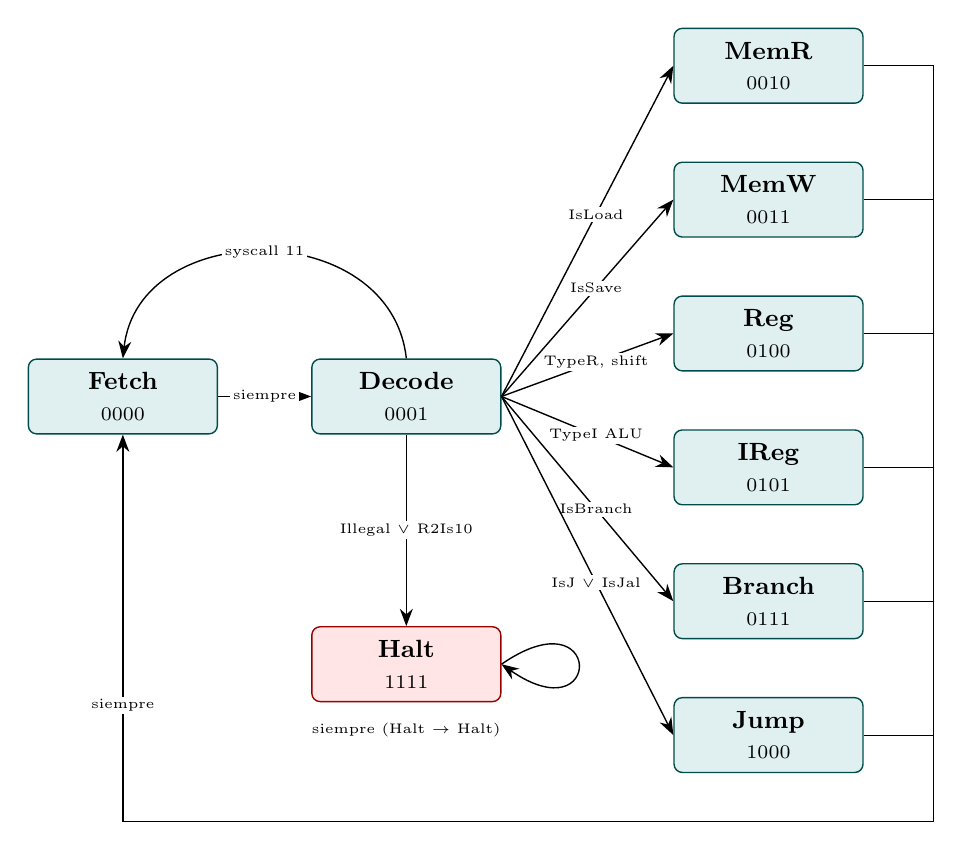
\begin{tikzpicture}[
  st/.style={draw,rounded corners=3pt,minimum width=2.4cm,minimum height=0.95cm,align=center,font=\small,line width=0.5pt,fill=teal!12,draw=teal!60!black},
  hs/.style={st,fill=red!10,draw=red!60!black},
  ar/.style={-{Stealth[length=2.2mm]},line width=0.5pt},
  lb/.style={font=\tiny,fill=white,inner sep=1pt}
]
\node[st] (f) at (0,0) {\textbf{Fetch}\\ \scriptsize 0000};
\node[st] (d) at (3.6,0) {\textbf{Decode}\\ \scriptsize 0001};
\node[st] (mr) at (8.2,4.2) {\textbf{MemR}\\ \scriptsize 0010};
\node[st] (mw) at (8.2,2.5) {\textbf{MemW}\\ \scriptsize 0011};
\node[st] (rg) at (8.2,0.8) {\textbf{Reg}\\ \scriptsize 0100};
\node[st] (ir) at (8.2,-0.9) {\textbf{IReg}\\ \scriptsize 0101};
\node[st] (br) at (8.2,-2.6) {\textbf{Branch}\\ \scriptsize 0111};
\node[st] (jp) at (8.2,-4.3) {\textbf{Jump}\\ \scriptsize 1000};
\node[hs] (h) at (3.6,-3.4) {\textbf{Halt}\\ \scriptsize 1111};
\draw[ar] (f) -- (d) node[lb,midway] {siempre};
\draw[ar] (d.east) -- (mr.west) node[lb,pos=0.55] {IsLoad};
\draw[ar] (d.east) -- (mw.west) node[lb,pos=0.55] {IsSave};
\draw[ar] (d.east) -- (rg.west) node[lb,pos=0.55] {TypeR, shift};
\draw[ar] (d.east) -- (ir.west) node[lb,pos=0.55] {TypeI ALU};
\draw[ar] (d.east) -- (br.west) node[lb,pos=0.55] {IsBranch};
\draw[ar] (d.east) -- (jp.west) node[lb,pos=0.55] {IsJ $\lor$ IsJal};
\draw[ar] (d.south) -- (h.north) node[lb,midway] {Illegal $\lor$ R2Is10};
\draw[ar] (h.east) .. controls +(1.3,0.9) and +(1.3,-0.9) .. (h.east);
\node[lb] at ([yshift=-0.35cm]h.south) {siempre (Halt $\to$ Halt)};
\draw[ar] (d.north) .. controls +(-0.2,1.8) and +(0.2,1.8) .. (f.north) node[lb,pos=0.5] {syscall 11};
\foreach \n in {mr,mw,rg,ir,br,jp} \draw (\n.east) -- (10.3,0 |- \n.east);
\draw (10.3,4.2) -- (10.3,-5.4) -- (0,-5.4);
\draw[ar] (0,-5.4) -- (f.south) node[lb,pos=0.3] {siempre};
\end{tikzpicture}
\caption{Diagrama de estados de la ControlUnit. Todo estado ejecutivo vuelve a Fetch; Halt es absorbente y tiene la m\'axima prioridad.}
\end{figure}

\subsection{Salidas por estado}
\begin{table}[H]
\centering
\small
\begin{tabular}{lllllp{5.2cm}}
\toprule
Estado & ASrc & BSrc & AluOp & AddrSrc & Otras se\~nales\\
\midrule
Fetch  & 1 & 1 & 0 & 0 & \sig{IRWrite}=1, \sig{PCWrite}=1\\
Decode & 0 & 0 & \sig{AluOp} & 1 & solo beq/bne usan 7; \sig{EnTTy} si syscall 11\\
MemR   & 0 & 2 & 0 & 1 & \sig{RegW}=1, \sig{Mem2Reg}=1, \sig{SaveReg}=1\\
MemW   & 0 & 2 & 0 & 1 & \sig{Reg2Mem}=1\\
Reg    & 0 (2 si shift) & 0 & \sig{AluOp} & 1 & \sig{RegW}=1, \sig{SaveReg}=0; jr: \sig{PCWrite}=1, \sig{isJr}=1, \sig{RegW}=0\\
IReg   & 0 (3 si lui) & 2 & \sig{AluOp} & 1 & \sig{RegW}=1, \sig{SaveReg}=1\\
Branch & 1 & 3 & 0 & 1 & \sig{PCWrite}=1, \sig{InBranchState}=1\\
Jump   & 1 & 1 & 0 & 0 & \sig{PCWrite}=1, \sig{JumpState}=1; jal: \sig{RegW}=1, \sig{SaveReg}=3\\
Halt   & -- & -- & -- & 1 & \sig{Halt}=1\\
\bottomrule
\end{tabular}
\caption{Salidas de la ControlUnit por estado. \sig{AddrSrc} llega al Datapath como \sig{PCsrc}.}
\end{table}

\begin{table}[H]
\centering
\small
\begin{tabular}{lll}
\toprule
C\'odigo & Mux A (\sig{ASel}) & Mux B (\sig{BSel}) \quad / \sig{SaveReg}\\
\midrule
0 & A (rs) & B (rt) \quad / rd\\
1 & PC & 4 \quad / rt\\
2 & shamt extendido & \sig{IValExt} \quad / (sin usar)\\
3 & 16 & \sig{IValExt}$\ll 2$ \quad / \$31\\
\bottomrule
\end{tabular}
\end{table}


\section{Cobertura de los programas de prueba}
\begin{table}[H]
\centering
\footnotesize
\begin{tabular}{@{}p{1.95cm}p{6.0cm}p{7.85cm}@{}}
\toprule
Instrucciones & Casos obligatorios & Programa(s) propios \\
\midrule
\sig{add}, \sig{sub} & Positivos y con al menos un operando negativo. & \sig{typer.asm} (add); \sig{burbuja.asm}, \sig{test\_printnum.asm} (sub); \\
\sig{and}, \sig{or} & Operandos con unos en los 16 bits altos. & \sig{custom\_testand.asm}, \sig{testandi.asm} (and); \sig{typer.asm} (or); \\
\sig{slt}, \sig{slti} & Resultado 1 y 0; negativo con signo distinto. & \sig{burbuja.asm} (slt con negativos); \sig{jaltest5.asm} (slti 1/0); \\
\sig{sll}, \sig{srl} & \sig{shamt}~$=0$ y $\neq0$; \sig{srl} con negativo. & \sig{sll.asm}, \sig{srl.asm} \\
\sig{addi} & Inmediato negativo. & \sig{sb.asm}, \sig{testlw.asm} \\
\sig{addiu}, \sig{addu} & Mediante \sig{li} y \sig{move}. & \sig{sll.asm}, \sig{srl.asm} (li); \sig{typer.asm} (addu); \sig{burbuja.asm} (move). \\
\sig{andi}, \sig{ori} & Inmediato con bit 15 a 1. & \sig{test\_ori.asm} (ori); \sig{lwzero3.asm} (andi con bit 15 a 0); \\
\sig{lui} & Inmediato con bit 15 a 1. & \sig{tlui.asm}, \sig{test\_lui.asm}, \sig{testandi.asm} \\
\sig{lw}, \sig{sw} & Desplazamiento positivo y negativo. & \sig{testlw.asm}, \sig{newlw.asm} (lw); \sig{sw\_sb.asm} (sw). \\
\sig{lb}, \sig{lbu} & Byte con bit 7 a 1 en al menos dos posiciones. & \sig{lb.asm} (lb, posición 0); \sig{lbsb2.asm} (lbu, 0--3); \\
\sig{sb} & Cuatro posiciones y comprobar con \sig{lw}. & \sig{sb.asm}, \sig{lbsb2.asm} (cuatro posiciones, comprobadas con \sig{lbu}); \\
\sig{beq}, \sig{bne} & Tomado y no tomado; al menos uno hacia atrás. & \sig{t09\_ramas.asm}, \sig{bnq.asm}, \sig{beq\_test.asm} \\
\sig{j} & Al menos una vez. & \sig{test\_jump.asm}, \sig{test\_branching.asm} \\
\sig{jal}, \sig{jr} & Procedimiento no hoja, \sig{\$ra} en la pila. & \sig{jaltest2.asm}, \sig{jaltest4.asm}, \sig{new2lw.asm} \\
\sig{syscall} & Servicios 11 y 10. & \sig{test\_syscall.asm} (y el resto de programas) \\
\sig{\$zero} & Escribir en \sig{\$zero} y comprobar que sigue a 0. & \sig{opozero.asm} \\
\bottomrule
\end{tabular}
\caption{Cobertura de los casos obligatorios con los programas propios de \sig{programs/} (sin los ejemplos entregados). Las filas parciales indican el caso que aún no se cubre.}
\end{table}

\end{document}
